\documentclass[11pt, oneside]{article}   	% use "amsart" instead of "article" for AMSLaTeX format
\usepackage{geometry}                		% See geometry.pdf to learn the layout options. There are lots.
\geometry{letterpaper}                   		% ... or a4paper or a5paper or ... 
%\geometry{landscape}                		% Activate for rotated page geometry
%\usepackage[parfill]{parskip}    		% Activate to begin paragraphs with an empty line rather than an indent
\usepackage{graphicx}				% Use pdf, png, jpg, or eps§ with pdflatex; use eps in DVI mode
% TeX will automatically convert eps --> pdf in pdflatex	
\usepackage{caption}
\usepackage{subcaption}
\usepackage{float}

\graphicspath{ {/home/linas/Desktop/kul/$em 2/advanced analytics in business/assignment 3/report/assets/}}	
\usepackage{amssymb}
\usepackage{listings}
\usepackage{xcolor}
\lstdefinestyle{mystyle}{
	basicstyle=\small\ttfamily,
	breaklines=true,
	frame=none,
	numbers=none,
	numberstyle=\tiny,
	numbersep=5pt,
	language=Python,
	captionpos=b,
	keywordstyle=\color{blue},
	commentstyle=\color{green!60!black},
	stringstyle=\color{blue},
	%backgroundcolor=\color{gray!10},
	xleftmargin=-5em, % Set the left margin to 0
}

\title{Assignment 3: \\ Predicting on streamed Steam reviews with Spark}
\author{\centering Ivo L. Arasin (r0926378) \and Vancesca Dinh (r0930510) \and Linas J. Leščinskas (r0874301) \and Yavuz Yavuzhan (r0920104)}
%\date{}							% Activate to display a given date or no date

\begin{document}
	\maketitle
	\section{Introduction}
	
	The goal of this assignment was to set up Spark and work in a streaming environment. This section briefly details the approach our group has taken to work with streaming data and is structured according to three key tasks of this assignment. 
	
	\section{Predicting on streamed textual data}
	
		\subsection{Construct a data set using the provided stream}
		Multiple group members took the effort to collect the streaming data from the provided endpoint. We have used 250 non-empty batches to construct the data set.
		First of all, we defined an empty dataframe (constructed from empty RDD) with schema to match the structure of JSON files that were received via streaming:
		
		\begin{lstlisting}[style=mystyle]
		# Define empty RDD
		empty_rdd = spark.sparkContext.emptyRDD()
		# Define schema for the dataframe
		columns = StructType([StructField('review_id', StringType(), False),
		StructField('app_id', StringType(), False), 
		StructField('review_text', StringType(), False), 
		StructField('label', StringType(), False)])
		# Create empty dataframe
		df = spark.createDataFrame(data=empty_rdd, schema=columns)
		df.show()
		\end{lstlisting}
		
		\noindent Then, we utilized a simple for-loop to go through directories and read in the received JSON files that contain Steam reviews. Some simple checks were performed to remove duplicate rows (in case several team members received the same batches) and remove empty reviews. Eventually, we constructed a data set that contains 793 rows. The class distribution was rather skewed, with 647 'positive' reviews and 146 'negative' reviews.
		
		\subsection{Construct a predictive model to predict the review target based on the review text}
		
		We split the data set into train and test portions, where 30\% is set aside for testing the model. Then we define a simple pipeline. 
		First, we separate words into tokens with RegexTokenizer, using any non-word character as a delimiter. Then, we remove stopwords with StopWordsRemover. In addition, we asked ChatGPT to generate a list of commonly used slang words in Steam reviews and appended that list to the one generated by the class. Then we consider two featurization approaches:
		
		\begin{itemize}
		\item \textbf{CountVectorizer}: to transform filtered words (tokens) into a matrix of token counts.
		\item \textbf{TF-IDF features}: to obtain a vector of weights that rewards frequently occurring words in a data set. We do not use external corpus to penalize frequently occurring words in a data set that also occur frequently in a given corpus.
		\end{itemize}
		
		\noindent Finally, we fit the logistic regression model (twice to consider both approaches).
		Model with CountVectorizer achieves 83\% accuracy, whereas TF-IDF model performs slightly worse, registering accuracy of 81\%.
		We save both models to a local directory so that they can be utilized for predictions as the stream comes in.
	
		
		\subsection{Use trained model to show you can make predictions as the stream comes in}
		In this step we adapt the provided notebook (\textit{spark\_streaming\_example\_predicting.ipynb}) to use the trained models for ‘live’ prediction of sentiment as the stream comes in. Essentially, we load the model from a local directory and apply it to a dataframe constructed from incoming JSON files. Then we select only relevant columns to display. 
		\vspace{11pt}
	
		\noindent Here we exhibit code and output of the model with CountVectorizer features:
		\vspace{11pt}
		
		\begin{lstlisting}[style=mystyle]
		# Add capability to predict as the stream comes in
		globals()['models_loaded'] = False
		globals()['my_model'] = None
		
		def process(time, rdd):
		if rdd.isEmpty():
		return
		
		print("========= %s =========" % str(time))
		
		# Convert to dataframe
		df = spark.read.json(rdd)
		df.show()
		# Load in the model if not yet loaded:
		if not globals()['models_loaded']:
		# load in your models here
		globals()['my_model'] = PipelineModel.load('/home/linas/Desktop/kul/$em 2/advanced analytics in business/assignment 3/model_tf_idf/')
		globals()['models_loaded'] = True
		# Make predictions with loaded model
		df_result = globals()['my_model'].transform(df)
		df_result.select("app_id", "label", "review_id", "review_text", "prediction").show()
		\end{lstlisting}
		
		\textbf{Example output:}
		
	\begin{figure}[h]
		\hspace{1cm} % Adjust the value to move the figure to the left
		%\centering
		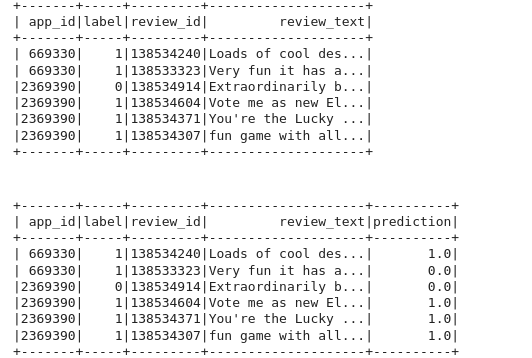
\includegraphics[width=1\linewidth]{output.png}
		\caption{Example output of predicting on streamed reviews}
		\label{figure label}
	\end{figure}
	
	We can see that the model stumbles on some instances and predicts the sentiment incorrectly. It is expected as it demonstrated imperfect accuracy on the test set as well. Model could be improved by constructing a larger data set, considering more sophisticated featurization and modeling approaches. However, achieving superior predictive performance was not the main goal of this assignment.	
	
	\section{Challenges}
	
	Throughout the work on this assignment, we encountered several challenges that we briefly detail below.
	\begin{itemize}
		
		\item Spark was generally very slow. It took 60 minutes to fit the pipeline on the training set and another 90 minutes to compute the accuracy of the model. Setting Spark to work with 4 cores (instead of 1 core as default) improved the situation. However, it was evident that Spark is not optimized to run on a single machine i.e. locally.
		\item Stream for receiving reviews kept continuously crashing after 3-4mins, necessitating a restart of the cell. Multiple group members were receiving the batches to alleviate the effort.
		
	\end{itemize}
	
\end{document}  